\section{Model architectures and training}
\label{sec:preliminary_work}

\paragraph{Motivation.}
\begin{figure}
	\centering
		
	\hfill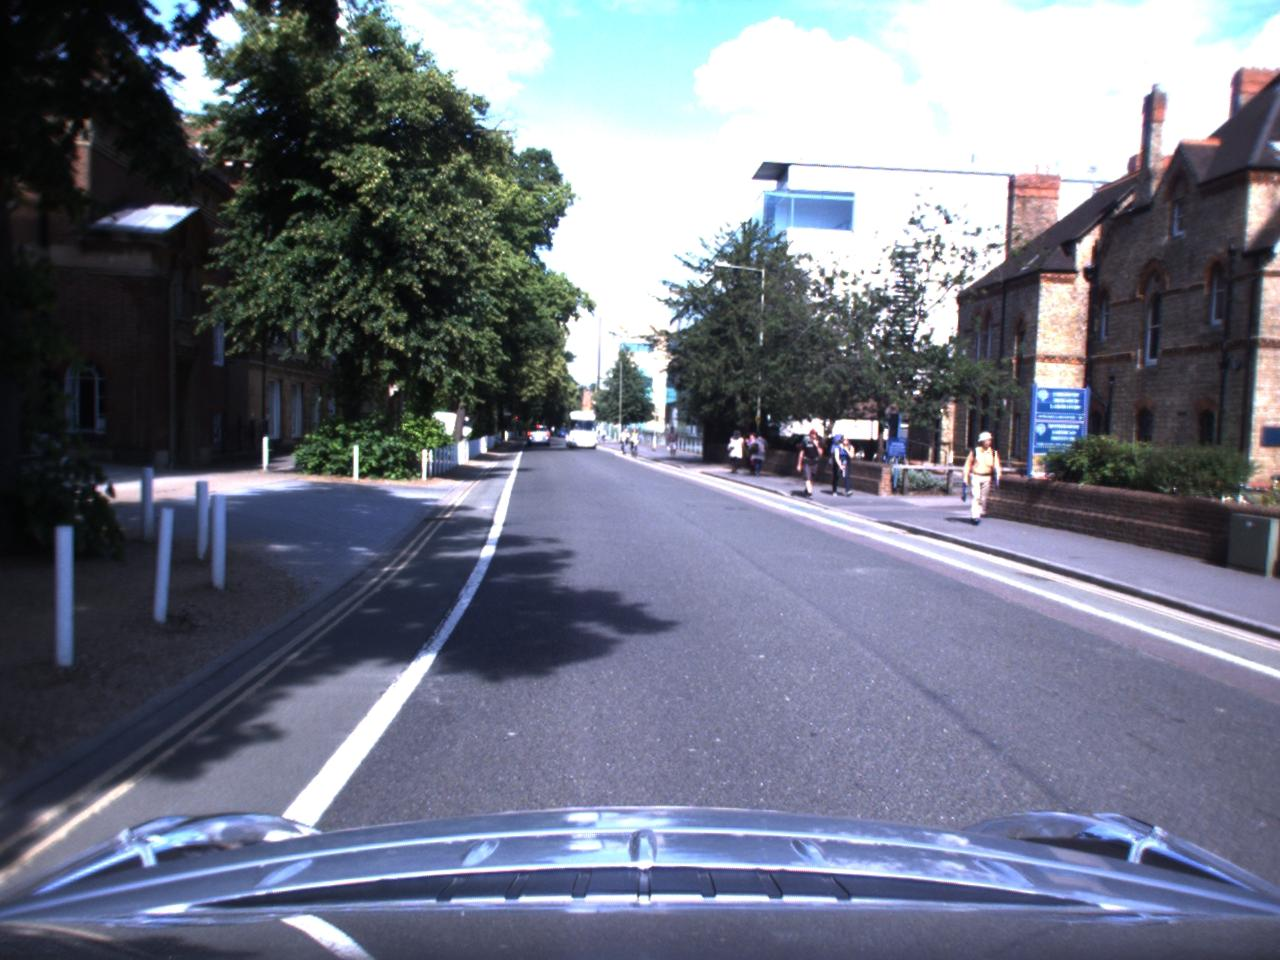
\includegraphics[width=0.25\linewidth]{preliminary/sun}\hfill
	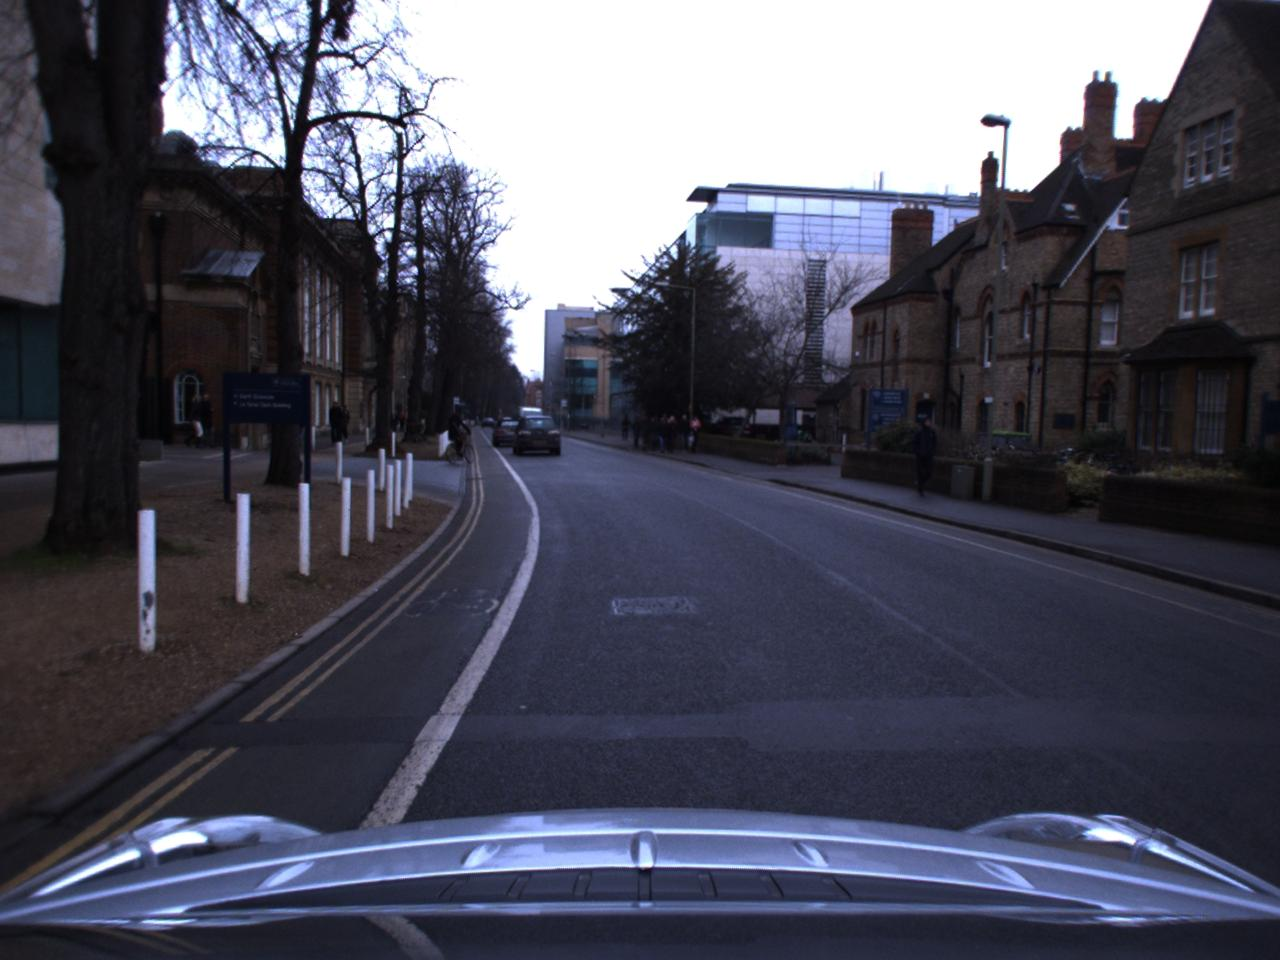
\includegraphics[width=0.25\linewidth]{preliminary/overcast}\hfill
	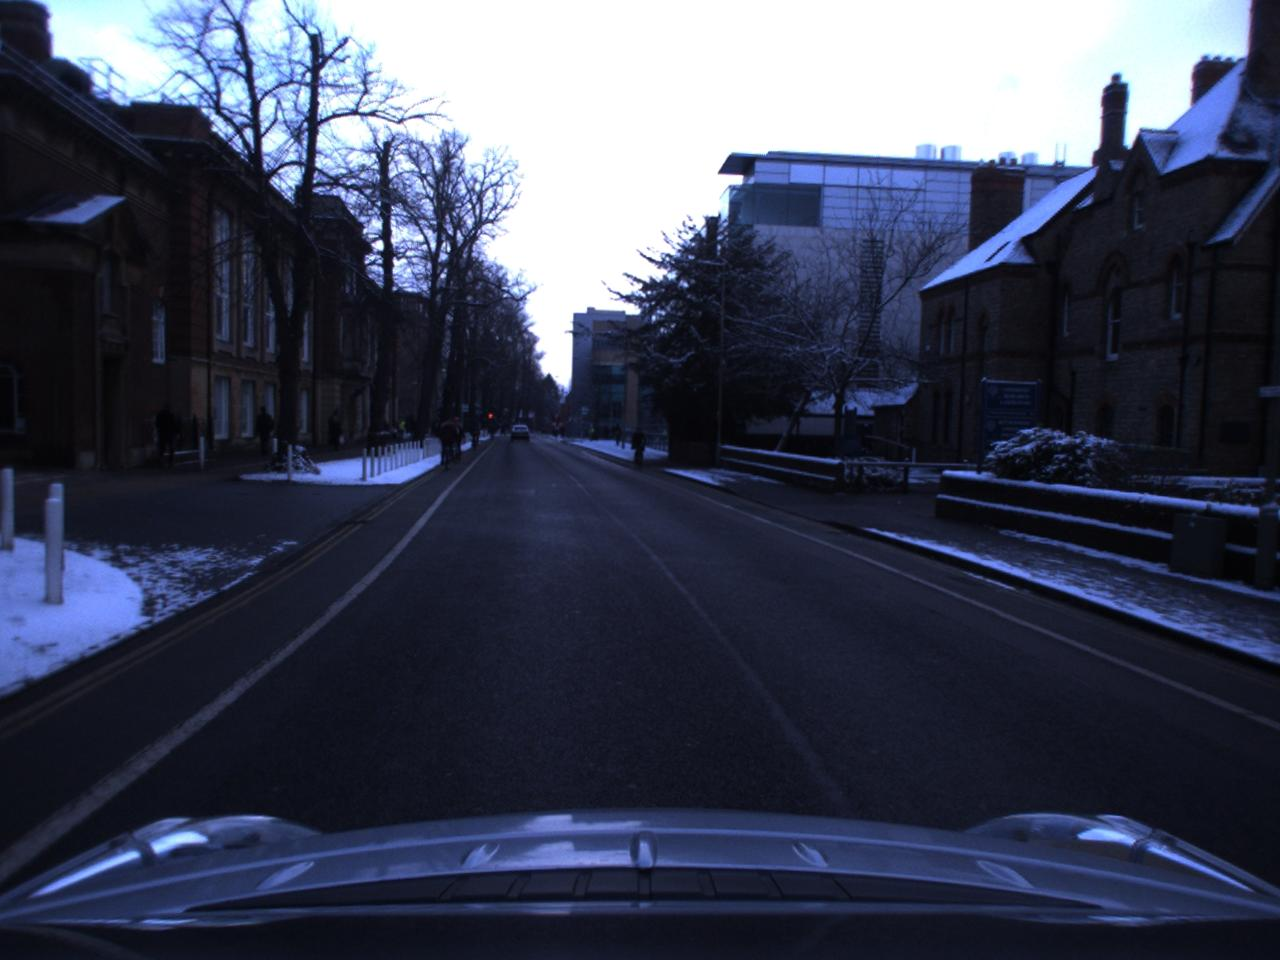
\includegraphics[width=0.25\linewidth]{preliminary/snow}\hfill
	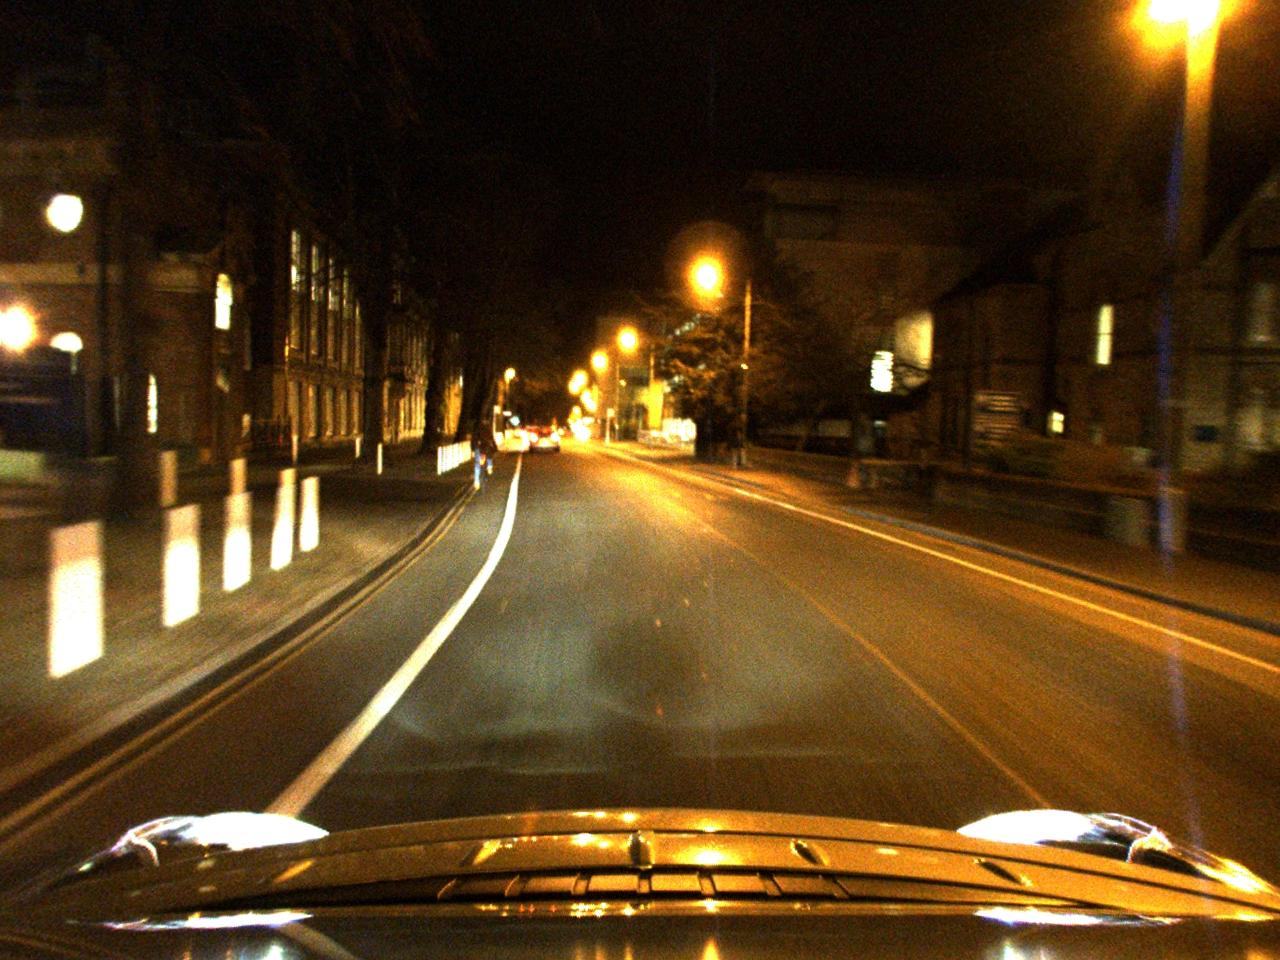
\includegraphics[width=0.25\linewidth]{preliminary/night}\hfill
	
	\hfill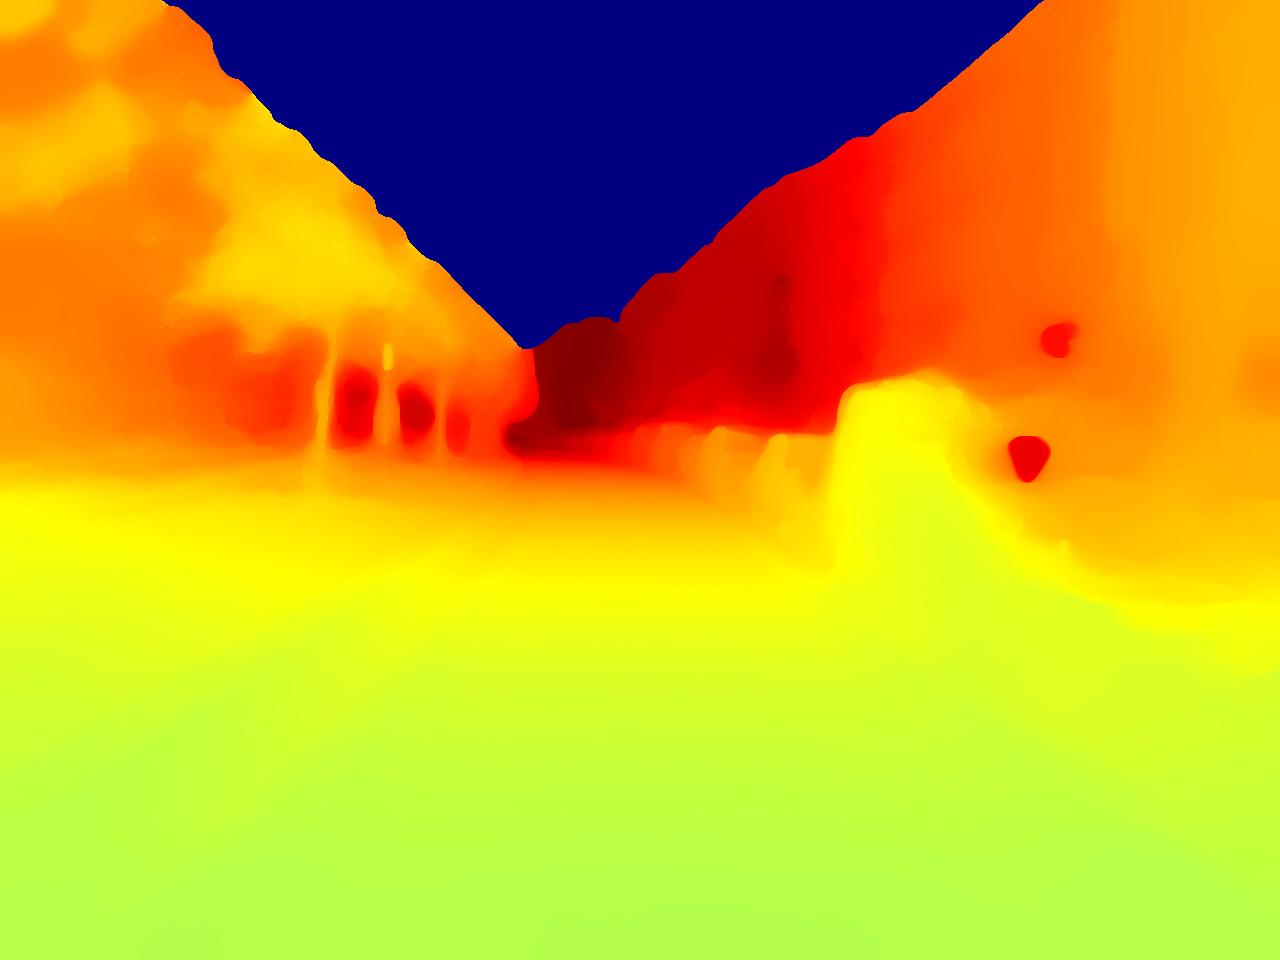
\includegraphics[width=0.25\linewidth]{preliminary/depth}\hfill
	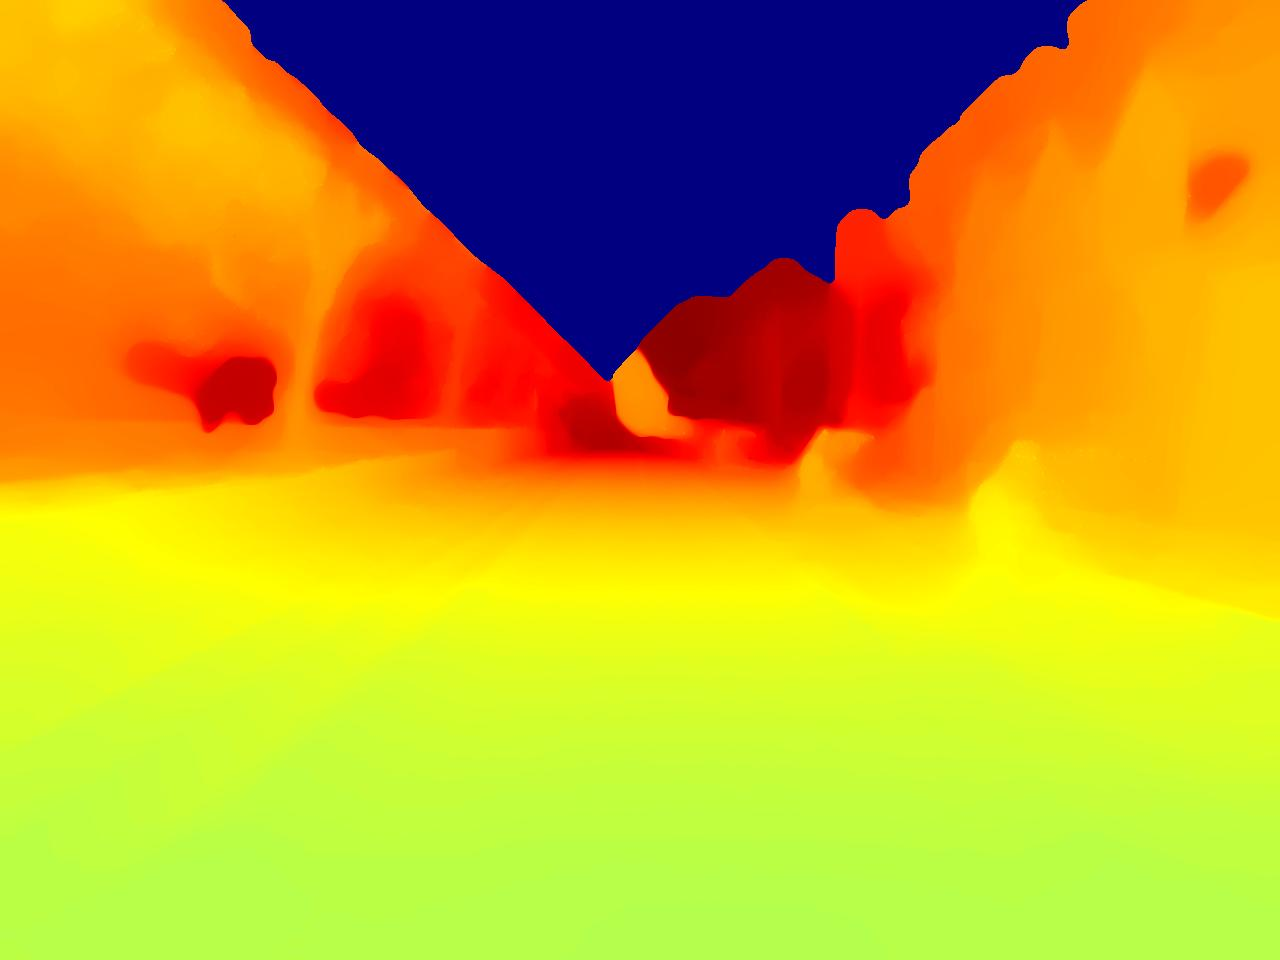
\includegraphics[width=0.25\linewidth]{preliminary/depth3}\hfill
	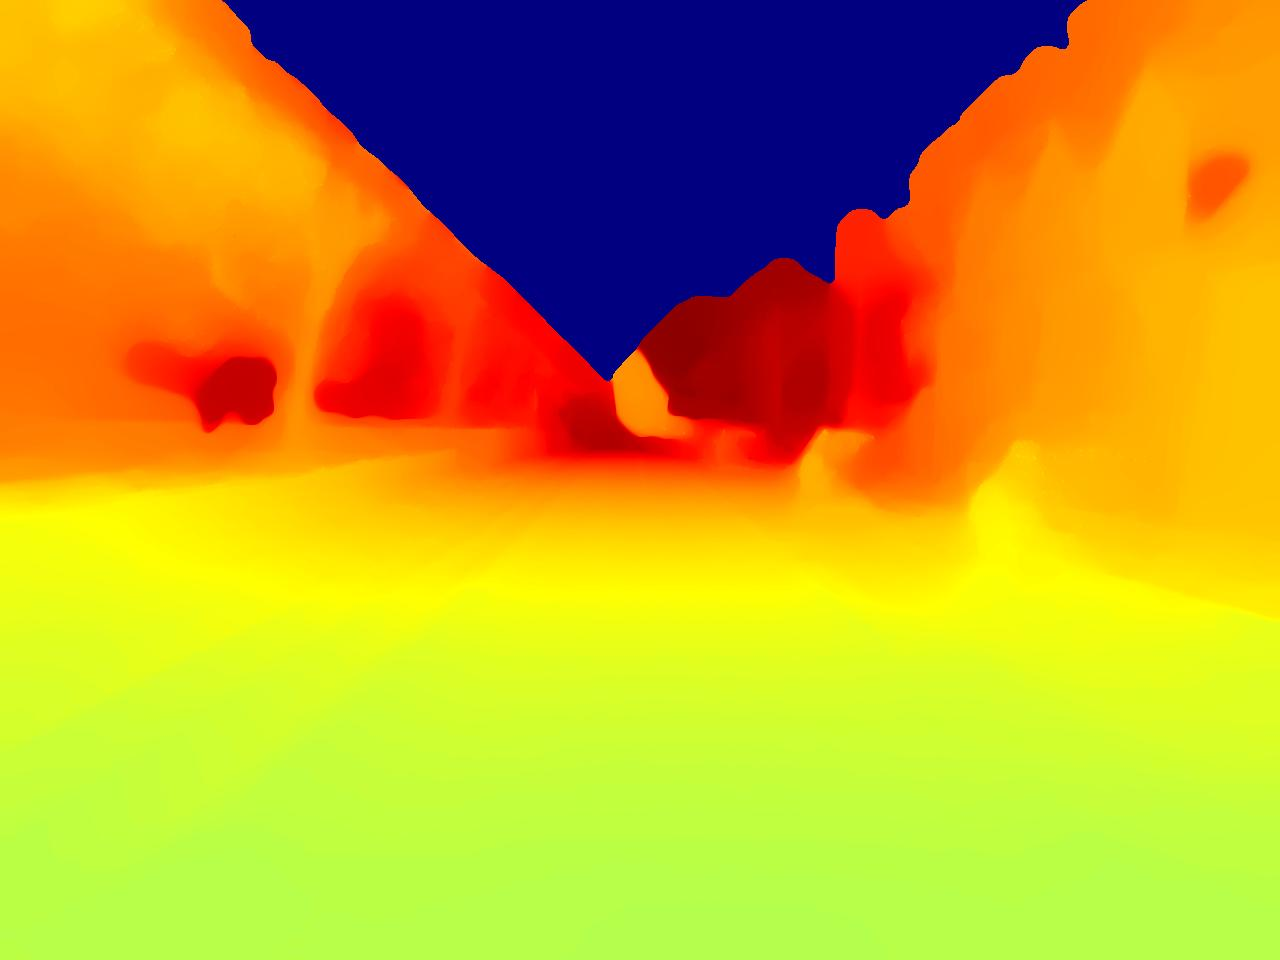
\includegraphics[width=0.25\linewidth]{preliminary/depth3}\hfill
	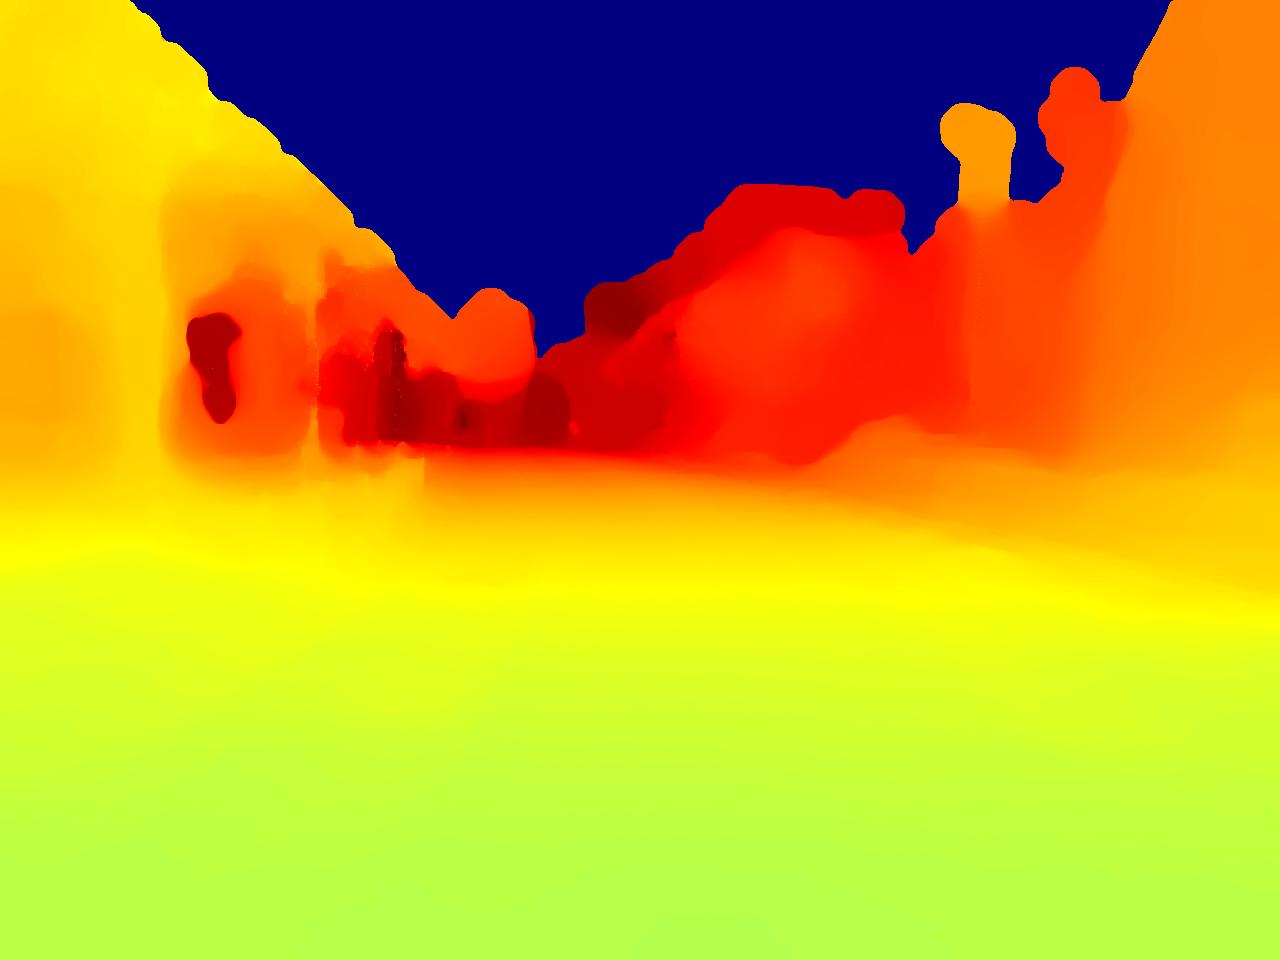
\includegraphics[width=0.25\linewidth]{preliminary/depth4}\hfill

	\caption[Images and depth maps comparison]{\label{fig:image_vs_depth} \textbf{Visual changes between radiometric and geometric domain:} due to outdoor conditions, visual aspect of images changes over time (top row), while, geometry of the scene (corresponding depth maps, bottom row) remains stable.}
	
\end{figure}
	
As illustrated in figure~\ref{fig:image_vs_depth}, outdoor conditions drastically impact visual appearance of a scene. It will be challenging for a descriptor relying only on the radiometric information to associate to the four images of figure~\ref{fig:image_vs_depth} similar embeddings. Thus, if we take a look at the underlying geometry in these images (\ie the associated depth maps, bottom of figure~\ref{fig:image_vs_depth}), this information seems more stable across changing conditions. The central idea of our method is to use recent modality transfer network~\citep{Eigen2014, Godard2017, Mahjourian2018} (from images to depth maps) to provide invariant image representation to our \ac{cnn} descriptor during training. At test time, the trained descriptor can be used on images only.

\subsection{Initial architecture}
\begin{figure}
	\centering
	
	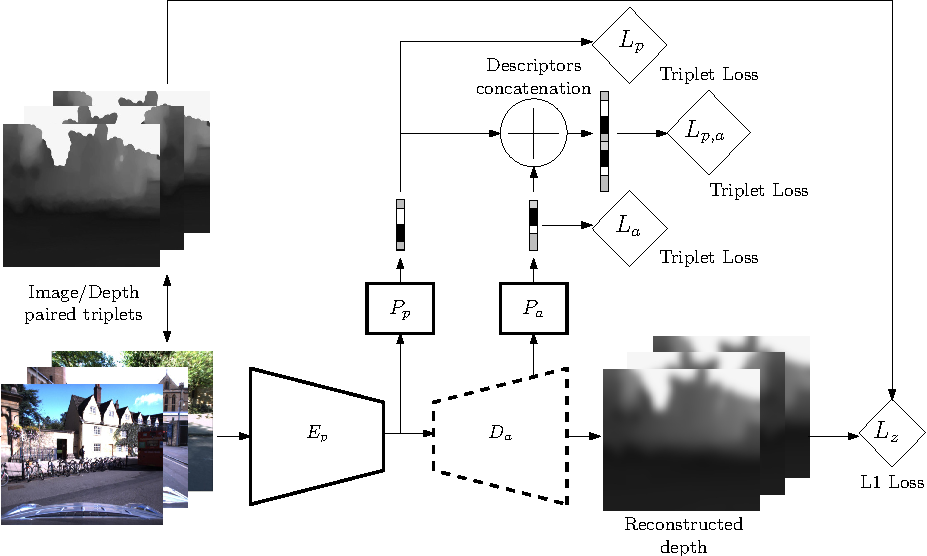
\includegraphics[width=\linewidth]{preliminary/preliminary_method}
	
	\caption[Preliminary solution]{\label{fig:preliminary_method} \textbf{Training pipeline of our preliminary solution.}}
	
\end{figure}
An overview of our method can be seen in figure~\ref{fig:preliminary_method}.

\paragraph{Principal descriptor.}
We build on recent advance in \ac{cnn} image descriptor for designing our system. We use standard convolution features extractor linked to a pooling descriptor layer (figure~\ref{fig:cnn_aggregation}). Formally, we denote $f_p$ the principal features vector of image $x$ computed by encoder $E_p$ and descriptor $P_p$:
\begin{equation}
	\label{eq:desc_details}
	f_p(x) = P_p(E_p(x)).
\end{equation}

We denote $\theta_{p}$ the weights of the image encoder and descriptor $\{E_p, P_p\}$. Notice that descriptor $P$ do not necessary contains trainable parameters (if we consider \ac{mac} pooling method for instance).

Considering the images triplet $\{x, x^+, x^-\}$, as described in previous section (see figure~\ref{fig:triplet_training}), our \ac{cnn} descriptor can be trained with the following triplet ranking loss~\citep{Arandjelovic2017}:
\begin{equation}
	\label{eq:triplet_loss}
	L_p(x, x^+, x^-) = max\left(\lambda + \norm{f_p(x) - f_p(x^+)}_2 - \norm{f_p(x) - f_p(x^-)}_2, 0 \right),
\end{equation}
where $\lambda$ is an hyper-parameter controlling the margin between positive and negative examples.

\paragraph{Side geometry learning.}
In order to recover the geometric information from the radiometric signal, we use a fully convolutional decoder $D_a$~\citep{Eigen2014}. $\theta_{a}$ are the trainable weights of our decoder. Lets $\{x, z\}$ be a pair of image and corresponding depth map, we can train our decoder to compute the depth map from input image with the following loss function:
\begin{equation}
	\label{eq:l1_loss}
    L_{pix}(x,z) = \norm{z - \hat{z}(x)}_{1},
\end{equation}
where $\hat{z}(x) = D_a(E_p(x))$, is the output of the decoder. $L_{pix}$ is a simple pixel loss penalizing absolute error between the output depth map $\hat{z}(x)$ and the target $z$.

\paragraph{Auxiliary descriptor.}
In order to take advantages of the learned depth representation in our final descriptor, we use intermediate deep features computed by $D_a$ to create another descriptor $f_a$:
\begin{equation}
	\label{eq:desc_aux}
	f_a(x) = P_a(\bar{D}_a(E_p(x))),
\end{equation}
where $P_a$ is an auxiliary descriptor and $\bar{D}_a$ designs an intermediate output extracted from decoder $D_a$. We do not use the reconstructed depth map $\hat{z}(x)$ (\ie raw output of $D_a$) to produce vector $f_a(x)$ because it will be to sensitive to small viewpoint variations. Instead, we use an intermediate output from $\bar{D}_a$, that should be more meaningful compared to  $\hat{z}(x)$ and less sensitive to viewpoint changes. Indeed, because the decoder upsample the feature maps, output of $\bar{D}_a$ has a smaller spatial resolution and is deeper in comparison to $\hat{z}(x)$. We apply a triplet ranking loss $L_a$ (see equation~\ref{eq:triplet_loss}) to train weights $\theta_{a}$ of decoder $D_a$ and descriptor $P_a$. 

\paragraph{Overall training.}
Finally, we combine the principal and auxiliary features, $f_p(x)$ and $f_a(x)$ in a common vector:
\begin{equation}
	\label{eq:concat_desc}
	f_{p,a}(x) = \left[ f_p(x), f_a(x)  \right],
\end{equation}
where $[ \cdot ]$ is the concatenation operation. Overall optimization is obtained through the last triplet ranking loss $L_{p,a}$ and the final optimization is defined by:
\begin{multline}
	\label{eq:overall_loss}
	\left( \theta_{p}, \theta_{a} \right) := arg\,\underset{\theta_p, \theta_a}{min} \left[ L_p(x, x^+, x^-) + L_a(x, x^+, x^-) + L_{p,a}(x, x^+, x^-) \right. \\
	\left. + \frac{1}{3}\left( L_{pix}(x, z) + L_{pix}(x^+, z^+) + L_{pix}(x^-, z^-) \right) \right].
\end{multline}

Our initial method requires triplets of RGB-D data to be trained.

\subsection{Hallucination network}
\begin{figure}
	\centering
	
	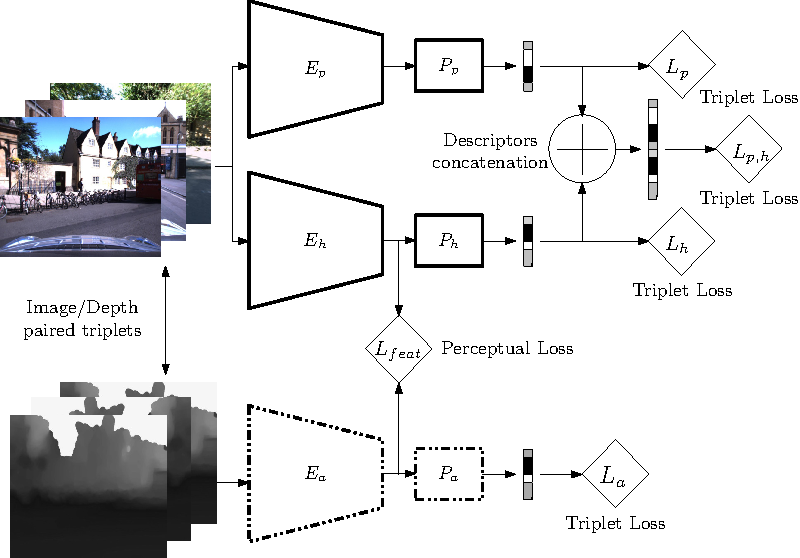
\includegraphics[width=\linewidth]{preliminary/hall_method_training}
	
	\caption[Hallucination network for image descriptors learning]{\label{fig:hall_method} \textbf{Hallucination network for image descriptors learning:} we train an hallucination network, inspired from~\cite{Hoffman2016}, for the task of global image description. Unlike the proposed method (see figure~\ref{fig:our_method}), hallucination network reproduces feature maps that would have been obtained by a network trained with depth map rather than the deep map itself.}
	
\end{figure}

We compare our method of side information learning with a state-of-the-art approach system, named hallucination network~\citep{Hoffman2016}. The hallucination network was originally designed for object detection and classification in images and have never tested for image description task. We adapt the work of~\citet{Hoffman2016} to create an image descriptor system that benefits from depth map side modality during training. Our adaptation of the hallucination network for image description is presented in figure~\ref{fig:hall_method}.

\paragraph{Principal descriptor.}
Similar to our proposal, the system is composed of a principal image descriptor: encoder $E_p$ + descriptor $P_p$, trained jointly through triplet ranking loss of equation~\ref{eq:triplet_loss}.

\paragraph{Auxiliary descriptor.}
Hallucination architecture needs an auxiliary network for training purpose, that will be discarded at test time. This auxiliary branch focus on extracting significant information from the side modality (the depth map in our case). We design the auxiliary network similar to our principal branch: the depth map descriptor is composed of an encoder $E_a$ linked to a descriptor $P_a$. The depth map descriptor is trained with a triplet ranking loss $L_a$, where the embeddings are directly computed from the truth depth maps:
\begin{equation}
	f_a(z) = P_a(E_a(z)).
\end{equation}

\paragraph{Hallucination descriptor.} The key component of \citet{Hoffman2016} proposal is the hallucination network. The task of the hallucination branch is, with images as input, to reproduce feature maps that would have been obtained by a network trained with depth map rather than the depth map itself. The hallucination network share the same architecture as the principal and the auxiliary branches. The hallucination descriptor is composed of an encoder $E_h$ and a descriptor $P_h$ with trainable weights $\theta_h$. It is trained with triplet ranking loss $L_h$ under the constraint of a perceptual loss~\citep{Johnson2016}:
\begin{equation}
	\label{eq:perceptual_loss}
	L_{feat}(x, z) = \norm{E_h(x) - E_a(z)}_2.
\end{equation}
This constraint can be interpreted as knowledge distillation~\citep{hinton2015distilling}. Final image descriptor is obtained by concatenating $f_p(x)$ and $f_h(x)$.

\paragraph{Overall training.} Training routine presented in~\citep{Hoffman2016} is two-step: we first train weights $\theta_a$ of the auxiliary descriptor with loss $L_a(z, z^+, z^-)$ and, secondly, we initialize hallucination weights $\theta_h$ with pre-trained weights $\theta_a$ and solve the following optimization:
\begin{multline}
	\label{eq:overall_hall_loss}
	\left( \theta_{p}, \theta_{h} \right) := arg\,\underset{\theta_p, \theta_h}{min} \left[ \alpha\left[ L_p(x, x^+, x^-) + L_h(x, x^+, x^-) + L_{p,h}(x, x^+, x^-) \right] \right. \\
	\left. + \gamma\left[ L_{feat}(x, z) + L_{feat}(x^+, z^+) + L_{feat}(x^-, z^-) \right] \right],
\end{multline}
where $\alpha$ and $\gamma$ are weighting constants. During final optimization, weights $\theta_a$ are frozen. 

Like our proposal, this method requires triplets of RGB-D data to be trained and, at test time, the principal and hallucination descriptors are used on images only.

\subsection{Discussion}
\label{subsec:discussion}
Exploratory testing of our method has lead to unsuccessful results. During the training step, our network failed to produce at the same time a meaningful image representation for localization (losses $L_p$, $L_a$ and $L_{p,a}$) and to reconstruct the scene geometry (loss $L_{pix}$). After analyzing our architecture, we came up with the following conclusions: the two target objectives are disrupting each other. This problem was due to the design of our method: error back-propagation from triplet ranking losses were affecting both weights of encoder $E_p$ and decoder $D_a$, as same as error computed by $L_{pix}$ in equation~\ref{eq:l1_loss}. 

We do not encounter the same problem with our implementation of hallucination network. The only loss functions that can interfere during the optimization are triplet ranking loss $L_h$ and perceptual loss $L_{feat}$. Both losses lead to modification of hallucination encoder $E_h$ weights. But targeted task of the two loss function are the same: $L_h$ directly optimize the hallucination embedding for image retrieval and $L_{feat}$ force the feature maps of encoder $E_h$ to be close to the feature maps of encoder $E_a$, an encoder that have been trained for image retrieval task as well.

In the next section, we propose an improved version of our initial method that solves the aforementioned issue.

\subsection{Final architecture}
\begin{figure}
	\centering
		
	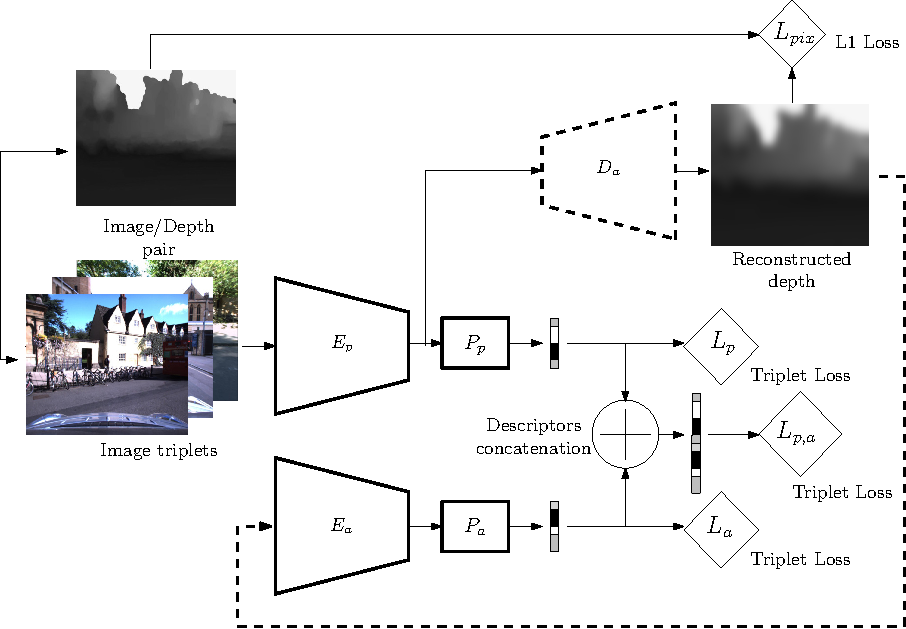
\includegraphics[width=\linewidth]{preliminary/our_method_training}
	
	\caption[Image descriptors training with auxiliary depth data]{\label{fig:our_method} \textbf{Image descriptors training with auxiliary depth data:} two encoders are used for extracting deep features map from the main image modality and the auxiliary reconstructed depth map (inferred from our deep decoder). These features are used to create intermediate descriptors that are finally concatenated in one final image descriptor.}
\end{figure}
	
Our modified architecture, presented in figure~\ref{fig:our_method}, is composed of:

\begin{itemize}
	\item a \ac{cnn} image encoder $E_p$ linked to a feature aggregation layer $P_p$ that produces the principal image descriptor,
	\item a \ac{cnn} image decoder $D_a$ used to reconstruct the corresponding depth map according to the monocular image,
	\item a \ac{cnn} depth map encoder $E_a$ linked to a feature aggregation layer $P_a$ that produces an auxiliary depth map descriptor,
	\item a fusion module that concatenates the image and depth map descriptor.
\end{itemize}

\paragraph{Training routine.}
\label{subsec:training}
Principal and auxiliary descriptor, $\{E_p, P_p\}$ and $\{E_a, P_a\}$, are trained separately with triplet ranking losses $L_p$ and $L_a$. As before, loss $L_{p, a}$ is used for joint optimization. The auxiliary descriptor $\{E_a, P_a\}$ takes as input the reconstructed depth map $\hat{z}(x)$. Similar to our first architecture, decoder $D_a$ take feature maps of encoder $E_p$ to generate output $\hat{z}(x)$. We constrain $\hat{z}(x)$ to be close to ground truth depth map $z$ with the pixel loss defined in equation~\ref{eq:l1_loss}. 

We designate $\theta_p$ weights of encoder/descriptor pair $\{E_p, P_p\}$,  $\theta_a$ weights of encoder/descriptor pair $\{E_a, P_a\}$ and $\theta_g$ weights of decoder $D_a$. The whole system is trained according to the following constraints:
\begin{align}
	\left( \theta_{p}, \theta_{a} \right) & := arg\,\underset{\theta_p, \theta_a}{min} \left[ L_p(x, x^+, x^-) + L_a(x, x^+, x^-) + L_{p,a}(x, x^+, x^-) \right], \label{eq:sys_optimization_1} \\ 	
	\left( \theta_{g} \right) & := arg\,\underset{\theta_{g}}{min} \left[ L_{pix}(x, z) \right]. 	\label{eq:sys_optimization_2}
\end{align}

We use two different optimizers: one updating $\theta_{p}$ and $\theta_{a}$ weights regarding constraint~(\ref{eq:sys_optimization_1}) and the other updating $\theta_{g}$ weights regarding constraint~(\ref{eq:sys_optimization_2}). Because decoder $D_a$ relies on feature maps computed by encoder $E_p$, at each optimization step on $\theta_p$ we need to update decoder weights $\theta_g$ to take in account possible changes in the image features. We finally train our entire system, by alternating between the optimization of weights $\{\theta_p, \theta_a\}$ and $\{\theta_g\}$ until convergence. By removing $E_p$ from the optimization of the depth from monocular objective (equation~\ref{eq:sys_optimization_2}) and by adding an auxiliary encoder $E_a$, we get rid of the interfering tasks problem observed earlier (see \S~\ref{subsec:discussion}). Notice that even if the encoder $E_p$ is not especially trained for depth map reconstruction, its intern representation is rich enough to be used by the decoder $D_a$ for the task of depth map inference.

\paragraph{Advantages and drawbacks.}
\label{paragraph:adv}
One advantage of the hallucination network over our proposal is that it does not require a decoder network ($D_a$), resulting in a architecture lighter than ours. However, it needs a pre-training step, where image descriptor $\{E_p, P_p\}$ and depth map descriptor $\{E_a, P_a\}$ are trained separately from each other before a final optimization step with the hallucination part of the system ($\{E_h, P_h\}$). Our system does not need such initialization. 

One advantage of our method over the hallucination approach is that we have two unrelated objectives during training: learning an efficient image representation for localization and learning how to reconstruct scene geometry from an image. It means that we can train several parts of our system separately, with different source of data. Especially, we can improve the scene geometry reconstruction task with non localized \textit{\{image, depth map\}} pairs. These weakly annotated data are easier to gather than triplet, as we only need calibrated system capable of sensing radiometric and geometric modalities at the same time. We will show in practice how this can be exploited to fine tune the decoder part to deal with complex localization scenarios in the following section~\ref{subsec:results}.

\subsection{Hard mining and swapping in triplet ranking loss}
\label{subsec:hard_minning}

\paragraph{Hard negative minning policy.} As mentioned in the previous section, hard mining is a crucial step in metric learning~\citep{Arandjelovic2017,Radenovic2017,Gordo2016,Iscen2018}. We construct our triplets like in~\citep{Arandjelovic2017}, using the GPS-tag information provided with the data. We gather $N$ triplets $\left\lbrace x, \left\lbrace x^+_i\right\rbrace_{i=1}^{M_p}, \left\lbrace x^-_i\right\rbrace_{i=1}^{M_n} \right\rbrace$ composed of one anchor, $M_p$ positive examples and $M_n$ negative examples. Negative examples are easy to find as we only have to consider all the data located further than a given distance threshold (according to the GPS information), resulting in a large number of examples ($M_n \approx 2000$ in our experiment). 

Because $M_n$ is too large, exact hard mining examples is not tractable. In~\citep{Arandjelovic2017}, authors store a fixed representation of the negatives examples that is used for negative mining. They update the representation of all negative examples as soon as the new representation computed by their model differ to much to the stored one. We adopt a different approach with a small overhead in term of computation but taking directly in account model updates. At each iteration, we randomly select a subset of $M_n^{sub}$ negative examples from the entire pool, and compute the truth hard negative example from this subset. This strategy also act as regularization during training as the negative training examples are different at each epoch.

\paragraph{Anchor and positive swapping.} We also adopt swapping technique introduced in~\citep{Balntas2016}. It simply consists of choosing the most confusing pair between \{anchor, negative\} and \{positive, negative\} examples:
\begin{multline}
\label{eq:triplet_loss_w_swap}
L^{swap}(x, x^+, x^-) = max\left(\lambda + \norm{f(x) - f(x^+)}_2 \right. \\
\left. - min\left(\norm{f(x) - f(x^-)}_2, \norm{f(x^+) - f(x^-)}_2 \right), 0 \right),
\end{multline}

\paragraph{Multiple examples.} Finally, we use all the positive examples and $M_n^{hard}$ hard negative mined examples from initial pool $M_n^{sub}$ of negative examples, to compute a normalized triplet ranking loss:
\begin{equation}
	L_{final}\left( x, \left\lbrace x^+_i\right\rbrace_{i=1}^{M_p}, \left\lbrace x^-_i\right\rbrace_{i=1}^{M_n^{sub}} \right) = \frac{1}{M_p M_n^{hard}} \sum_{i=1}^{M_p} \sum_{j=1}^{M_n^{hard}} L^{swap}\left( x, x^+_i, x^-_j \right).
\end{equation}

\subsection{Descriptors fusion and dimension reduction}
\begin{figure}
	\centering
		
	\begin{minipage}{0.65\linewidth}		
		\centering
		
		\begin{minipage}{0.5\linewidth}
			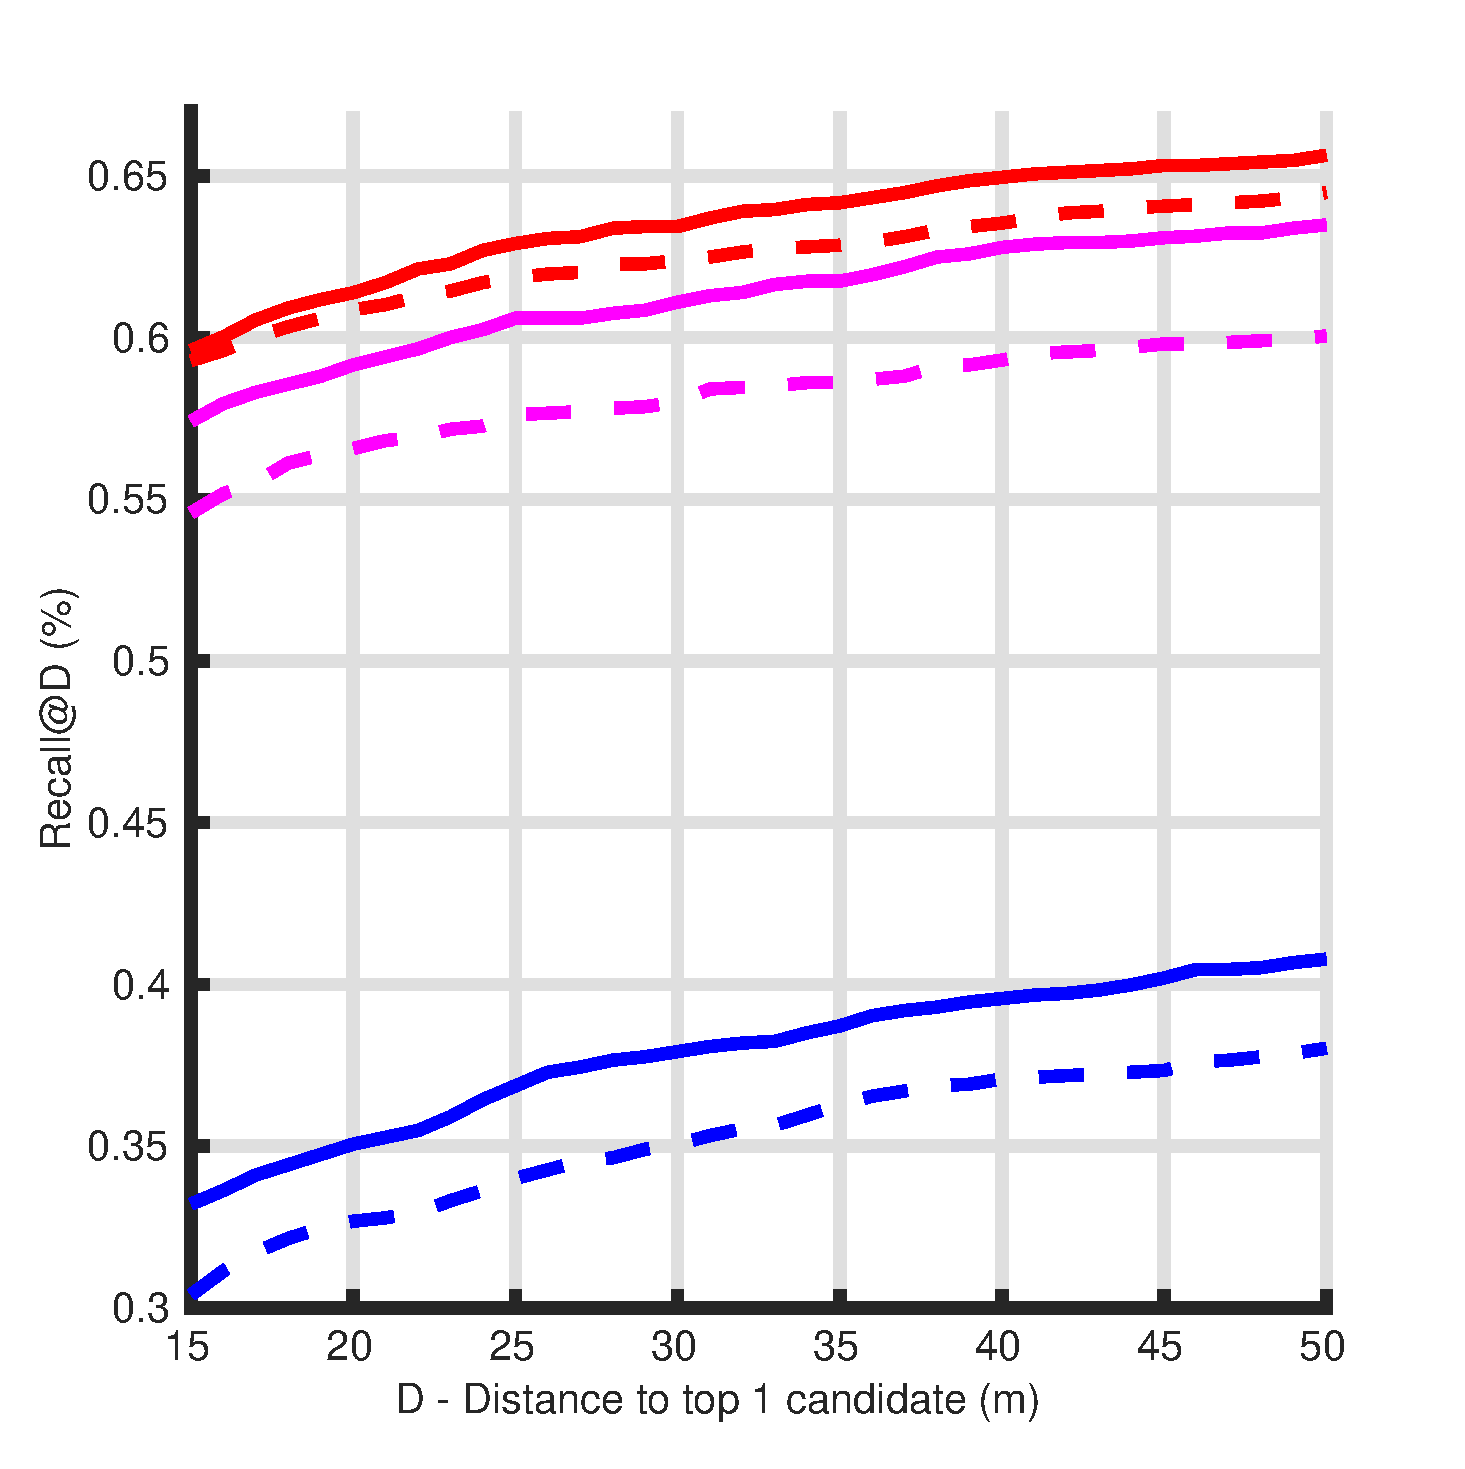
\includegraphics[width=\linewidth]{preliminary/joint_distance}
		\end{minipage}\hfill
		\begin{minipage}{0.5\linewidth}
			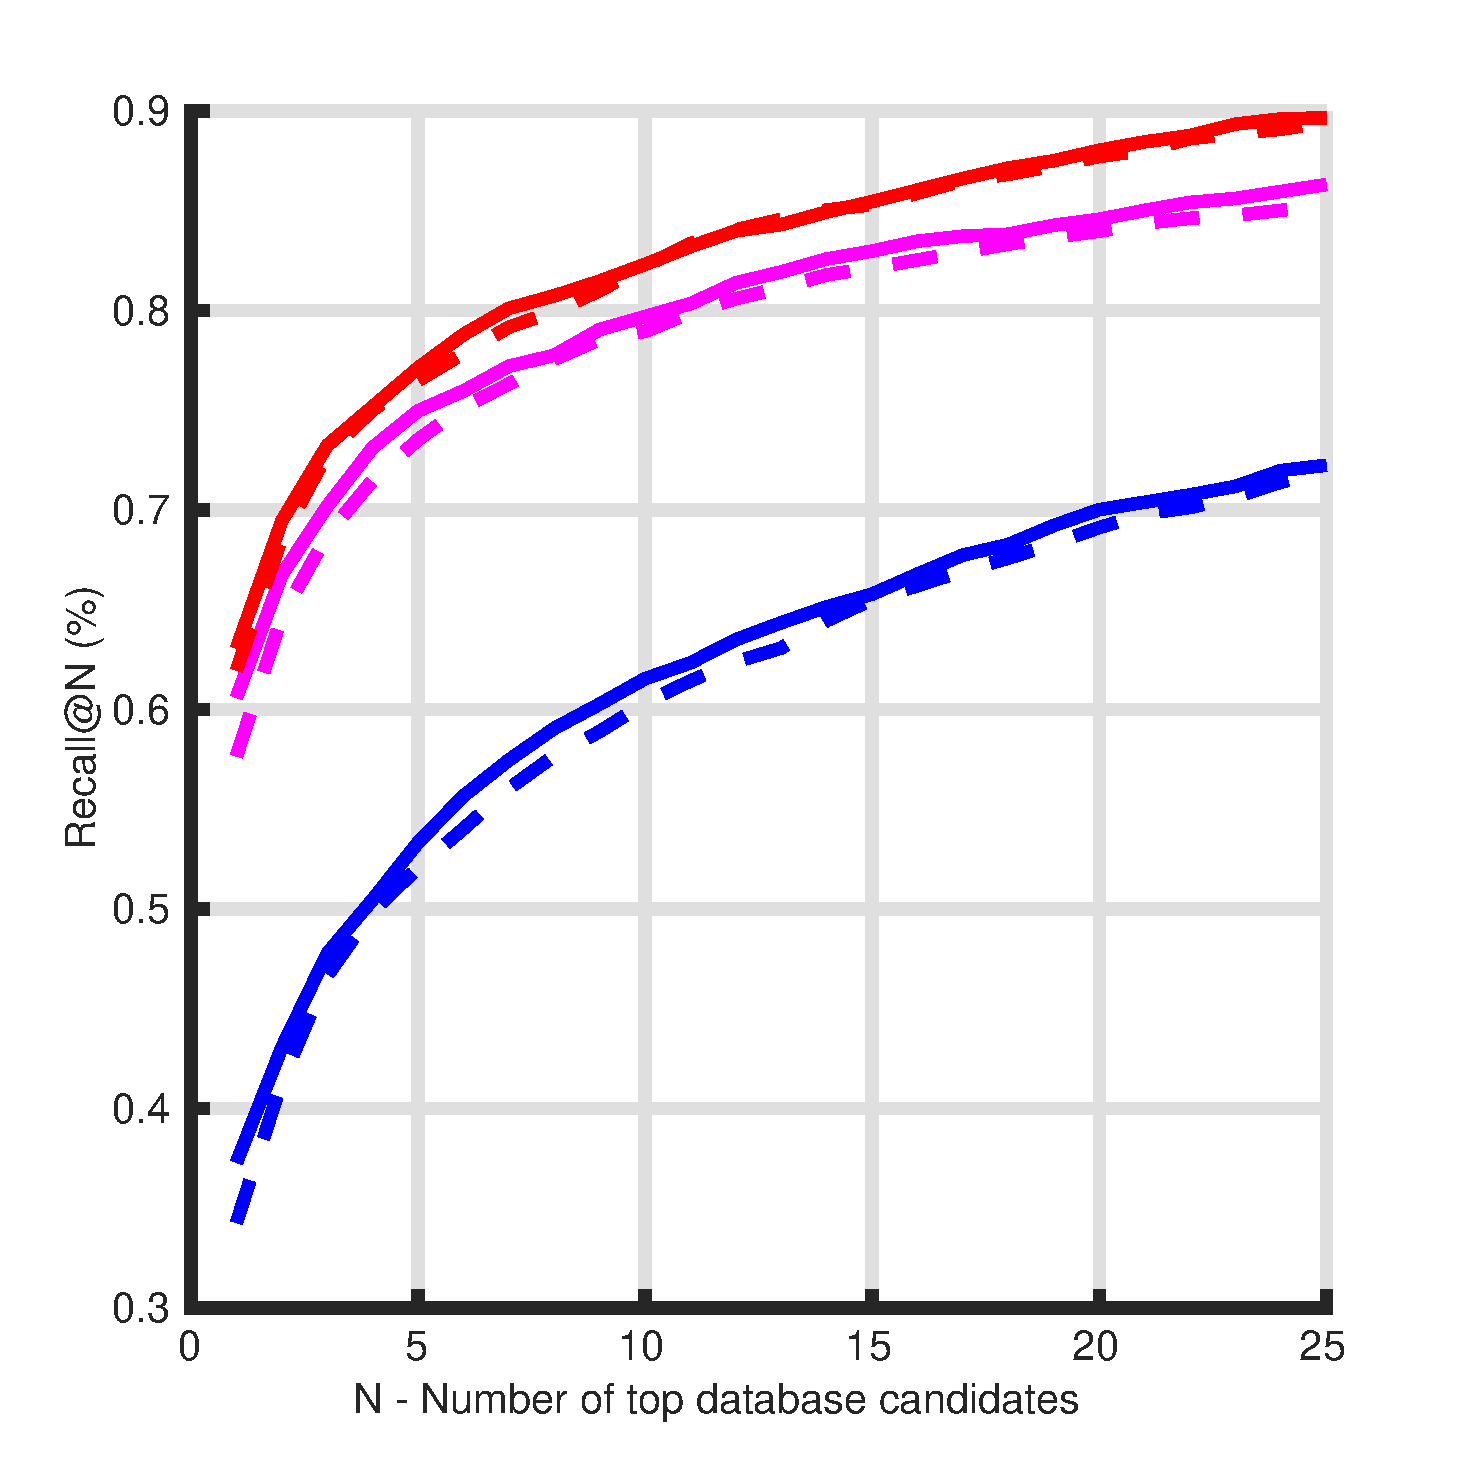
\includegraphics[width=\linewidth]{preliminary/joint_recall}
		\end{minipage}
		
		\vspace{0.2cm}
		
			\setlength{\tabcolsep}{2pt}
			\begin{tabular}{c l c l}
				\Large{- -} & Individual optimization & \textbf{\Large{--}} & Joint optimization \\
			\end{tabular}			
			
			\begin{tabular}{c c c c}
				Test set: & \textcolor{red}{{--} CMU--LT} & \textcolor{magenta}{{--} CMU--Autumn} & \textcolor{blue}{{--} CMU--Snow} \\
			\end{tabular}			
		
	\end{minipage}\hfill
	\begin{minipage}{0.35\linewidth}
		\caption[Joint vs individual optimization]{\label{fig:fuse_desc} \textbf{Influence of the joint loss $L_{p,a}$:} we report localization results of our method trained with or without the joint triplet ranking loss $L_{p,a}$. We detail the used metrics and datasets in section~\ref{sec:impl_details}.}
	\end{minipage}	

\end{figure}
	
\label{subsec:fuse_desc}
\paragraph{Fusion policy.}
We try to replace our basic features fusion operator introduced in equation~\ref{eq:concat_desc} (vectors concatenation) by more advanced functions, in order to benefit as much as possible from the complementarity of the principal and the auxiliary modalities. We investigate: hand-tuned descriptors scalar weighting, trained scalar weighting~\cite{Sizikova2016}, trained modal attention mechanism at the level of descriptors and trained spatial and modal attention mechanism at the level of the deep features~\cite{Seymour2018}. We found that all the fusion policies perform similarly. Indeed, as you can see in figure~\ref{fig:fuse_desc}, the modalities fusion are learned by our system through the triplet loss $L_{p, a}$, making the system aware of what is important and complementary in the radiometric and geometric domain, without the need of a complex fusion method.

\paragraph{Post-treatment.}
We reduce the dimension of the final descriptor by applying PCA + whitening~\citep{Arandjelovic2017, Radenovic2016, Radenovic2017, Gordo2017}. After the convergence of the whole system we reuse the images from the training dataset to compute the PCA parameters.